The training mode is an optional step which can be perfomed after the planning stage has been completed.
In training mode, users can play through previously planned procedures step by step by following the instructions found in the virtual OT and performing individual procedure steps.
Users are able to familiarize themselves with the steps and tools necessary for specific procedures.
Additionally, visualization tools can be utilized to understand patient's anatomy, pathology and instrument placement at each procedure step.
Instructions, mainly about which procedure has to be performed with which respective tools, are shown.
The steps and instructions depend on the project case, which includes saved procedure steps.
Additional information for each individual step can be added by simply modifying the project cases text in the JSON file.
The basic flow of interaction in this mode is depicted in Figure \ref{fig::TrainingFlow}.

\begin{figure}[ht]
    \centering
    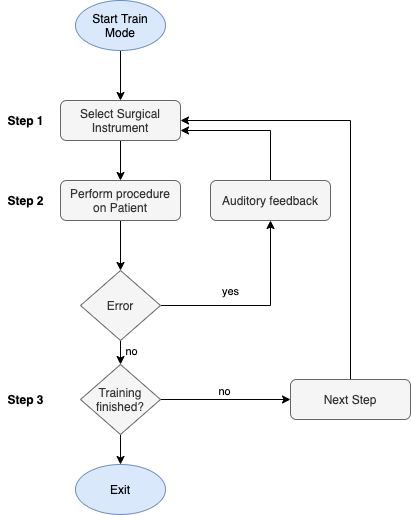
\includegraphics[width=225px]{images/implementation/features/training/training_flow.png}
    \caption{\label{fig::TrainingFlow}Simplistic Flow during Training Stage}
\end{figure}

\textbf{Step 1}: Users read the textual information and get a sense of which procedure step is to be performed.
They then pick up an instrument. In case of the drilling procedure, the correct drill bit has to be chosen.
When performing a hammer procedure, the correctly sized chisel has to be chosen.
In case of the osteosynthesis plates, the correct plate has to be chosen.
Drill bits, chisels and plates are labeled so that users know which one to pick.
Correctness of the procedure is checked in the following step.

\begin{figure}
    \centering
    \begin{minipage}{.5\textwidth}
      \centering
      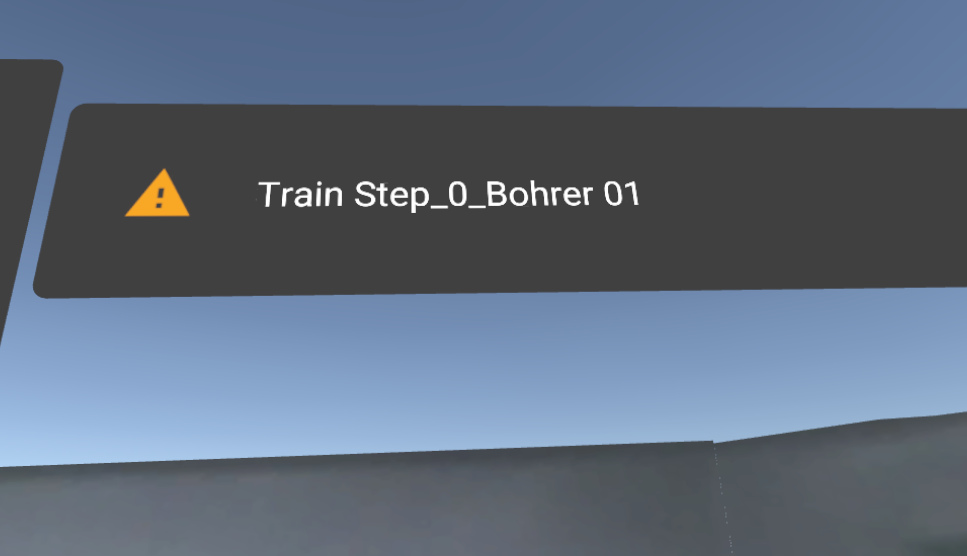
\includegraphics[width=0.95\linewidth]{images/implementation/features/training/train_guide.png}
    \end{minipage}%
    \begin{minipage}{.5\textwidth}
      \centering
      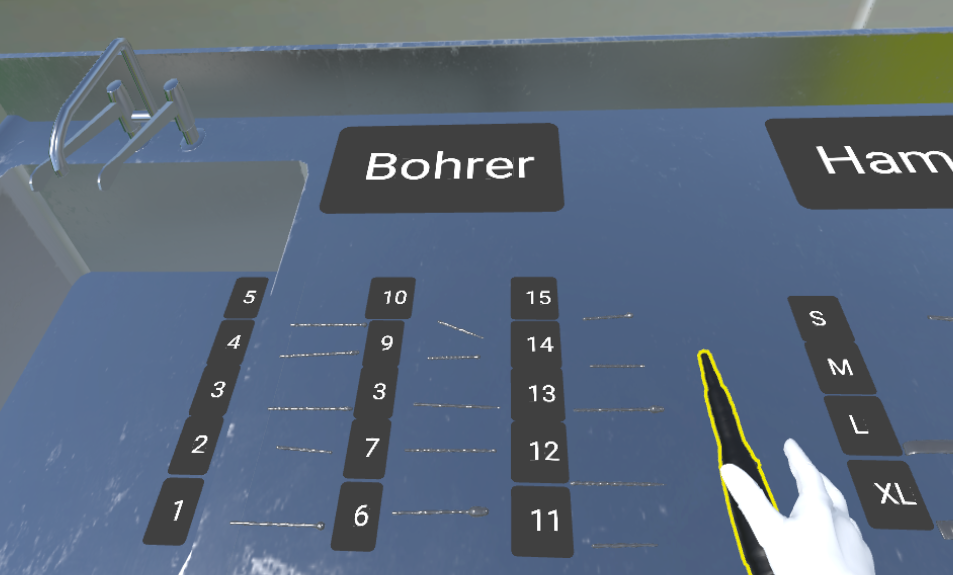
\includegraphics[width=0.915\linewidth]{images/implementation/features/training/train_select.png}
    \end{minipage}
    \begin{minipage}{1\textwidth}
        \centering
        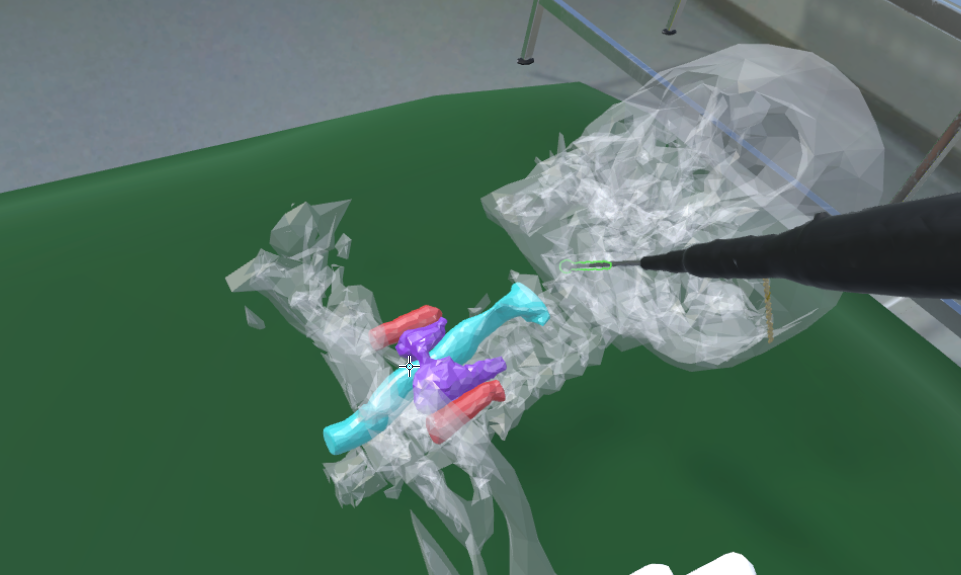
\includegraphics[width=0.95\linewidth]{images/implementation/features/training/training.png}
      \end{minipage}%
    \caption{\label{fig::TrainingMode}Training guidance and assistance, TODO ANDREA: IMPROVE THIS}
  \end{figure}

\textbf{Step 2}: The current step which is to be perfomed will also be hinted at in the patient's 3D model (Figure \ref{fig::TrainingMode}).
The outline of the current step is shown to the user, and the correct procedure has to be applied at the surgical site in which the outline is shown to progress.
Correctness is checked by measuring if the involved surgical instruments are overlapping with the current procedure step.
Additionally, since all surgical instruments are labeled, the label will also be checked.
If an error has been made (i.e. wrong attachment or wrong location), voice feedback is given and the user has to retry the procedure.
In the case of success, the voice feedback will signal that the next step is to be performed and the instructions and outline of the step will change accordingly.

\textbf{Step 3}: If all steps have been finished, the training mode will finish and the planning mode will resume.
